\pdfoutput=1 % only if pdf/png/jpg images are used
\documentclass{JINST}

\usepackage{amsmath,amssymb}
\usepackage[numbers]{natbib}
%\usepackage{hyperref}
%\hypersetup{colorlinks, citecolor=blue, linkcolor=blue, filecolor=blue, urlcolor=red}

\title{Improved Background Rejection in Neutrinoless Double Beta Decay Experiments with Gaseous Xenon Detectors}

\author{A. Author$^a$,
B. Author$^a$\thanks{Corresponding author.}~
and C. Author$^b$\\
\llap{$^a$}Instituto de F\'isica Corpuscular (IFIC), CSIC \& Universitat de Val\`encia,\\ 
Calle Catedr\'atico Jos\'e Beltr\'an, 2, 46980 Paterna, Valencia, Spain\\
\llap{$^b$}Name of Institute,\\
  Address, Country\\
E-mail: \email{CorrespondingAuthor@email.com}}

\bibliographystyle{plainnat}

\abstract{We propose a potential improvement in background rejection capability of neutrinoless double-beta ($0\nu\beta\beta$) decay experiments conducted with high-pressure xenon gas detectors capable of imaging electron tracks.  The improvement relies on the ability to distinguish the different track signatures left by single-electron (background) events and two-electron ($0\nu\beta\beta$) events in such a detector in the presence of an external magnetic field.  This initial study shows that, by analyzing the curvature of the reconstructed helical tracks, a potentially significant additional background rejection factor can be obtained with an acceptable loss in signal efficiency.}

\keywords{Neutrinoless double beta decay; Kalman filter; particle tracking}

\begin{document}

\section{Introduction}\label{sec:intro}
The observation of neutrinoless double-beta ($0\nu\beta\beta$) decay, in which two simultaneous $\beta$-decays occur within a nucleus resulting in two emitted electrons and no emitted neutrinos, would have several significant implications in fundamental physics.  First, the decay cannot occur unless the neutrino is a Majorana particle, that is, unless it is physically equivalent to its anti-particle.  Majorana neutrinos would be evidence for new physics at an energy scale inversely proportional to the neutrino masses and their existence violates the conservation of total lepton number.  Lepton number violation combined with CP violation could explain the excess of matter over anti-matter present in the universe.

Many experimental challenges accompany these far-reaching physics implications.  No confirmed observation of $0\nu\beta\beta$ has yet been made, and detectors with over 100 kg of candidate isotope have been constructed.  Thus it may be necessary to design an experiment capable of operating with tonnes of candidate isotope.  High pressure xenon detectors offer technology that could potentially allow operation at the ton-scale and permit the reconstruction of ionization tracks with good resolution.  

The energetic electrons produced in $0\nu\beta\beta$ decay deposit their energy as they travel through the xenon gas,
leaving a track of ionization in their path.  Because the ionization density $dE/dx$ is greater at lower electron energies,
the two ends of the electron tracks are marked by two ``blobs'' of greater ionization density.  For a single-electron
track, only one ionization track with one ``blob'' is produced.  This difference in track signatures can be used to
distinguish between background events, for example due to high-energy gamma rays, that produce single-electron
tracks, and double-beta events.\footnote{Note that this track signature is present for both $0\nu\beta\beta$ and
$2\nu\beta\beta$ events, and so it cannot be used to reject background events from the two-neutrino mode.  For this
one must rely on good energy resolution.}  Such studies based on identification of the two ``blobs'' have already shown
that the track signatures can be used to reject background events.  In this study we compare the single and
double-electron track signatures in the presence of an applied external field and quantify the additional ability to 
reject single-electron events that is gained by examining the curvature of the tracks induced by the field.

%The $0\nu\beta\beta$ experiment NEXT will use 100 kg of xenon enriched in the candidate isotope $^{136}$Xe in a
%high pressure xenon time projection chamber (TPC).  A tracking plane consisting of silicon photomultipliers (SiPMs)
%will be used to reconstruct ionization tracks in $(x,y)$, while the $z$-coordinate is determined using the drift time of
%electrons in a readout scheme based on electroluminescence (EL).  A resolution in $(x,y,z)$ of several mm is anticipated,
%and therefore the techniques developed here should be directly applicable to such an experiment.

\section{Particle Tracks in Xenon in a Magnetic Field}\label{sec:magmotion}
A particle of charge $q$ moving at a velocity $\mathbf{v}$ in the presence of a magnetic field $\mathbf{B}$ is acted 
upon by a force

\begin{equation}
\mathbf{F} = q(\mathbf{v} \times \mathbf{B}).
\end{equation}

This force will cause an electron to execute helical motion in the magnetic field such that if the thumb of the right hand is positioned along the direction of the field line $\mathbf{B}$ the electron will spiral in the direction in which the fingers curl when closed around the field line (see figure \ref{fig_bfieldmotion}).  The frequency of rotation about the field line is known as the cyclotron frequency $\omega_{\mathrm{cyc}} = qB/m$, where $B$ is the magnitude of the applied magnetic field $B = |\mathbf{B}|$ and $m$ is the mass of the charged particle.
% radius of curvature $r = p_{T}/qB$

\begin{figure}[!htb]
	\centering
	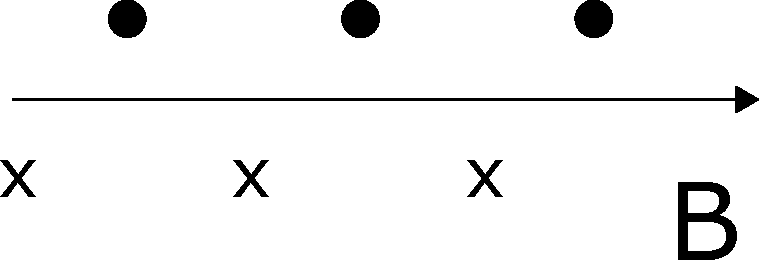
\includegraphics[scale=0.48]{fig/bfield_motion.pdf}
	\caption{\label{fig_bfieldmotion}Motion of an electron in a magnetic field.  The electron exhibits helical motion around the field line as shown (entering the page at the $\times$ and exiting the page at the $\bullet$) regardless of the direction of the component of the electron's velocity along the direction of $\mathbf{B}$.}
\end{figure}

In the presence of an applied external magnetic field, the ionization track produced by an energetic electron moving 
through high pressure xenon gas will be a helix with some alterations due to electron multiple scattering.  If the direction
of the applied magnetic field is known, the curvature of the track can be calculated to determine whether the component
of the electron velocity along the magnetic field is parallel or antiparallel to the field.  The curvature $\kappa$ can 
be calculated for track coordinates $(x,y,z)$ as

\begin{equation}\label{eqn_curv}
\kappa = \frac{(dx/dz)\cdot(d^2y/dz^2) - (dy/dz)\cdot(d^2x/dz^2)}{\Bigl[(dx/dz)^2 + (dy/dz)^2\Bigr]^{3/2}}.
\end{equation}

With this definition, an electron traveling in the direction of the magnetic field will spiral around the field lines with positive curvature, while an electron traveling opposite the direction of the magnetic field will spiral with negative curvature.  The curvature, however, will be of the opposite sign if the track orientation is not properly identified in the calculation (i.e., if $dz$ is of the wrong sign).  Thus, when calculating the curvature of a single-electron track, one would expect $\kappa > 0$ for $dz > 0$ and $\kappa < 0$ for $dz < 0$ given that $dz$ is always in the direction of the electron velocity.  However, for a $0\nu\beta\beta$ track, taking one of the extremes to be the beginning of the track and the other to be the end will lead to a calculation of $\kappa$ assuming the wrong track orientation for one of the two electrons, as the vertex at which the reaction occured is found somewhere on the interior of the track.  Therefore one expects to find $\kappa < 0$ for $dz < 0$ and $\kappa > 0$ for $dz > 0$ for a significant fraction of the track.  This difference in the behavior of the calculated curvature of reconstructed tracks will allow for the separation of single-electron and $0\nu\beta\beta$ events.

\section{Implementation}

\subsection{Track Preparation}\label{ssec:track}
The simulation-based study consisted of analysis of Monte Carlo datasets generated in a large virtual box of high pressure xenon gas using GEANT4.  For various configurations of gas pressure and magnetic field, 10000 events were generated consisting of single energetic electrons of kinetic energy equal to the Q-value of $0\nu\beta\beta$ in xenon gas ($Q_{\beta\beta} = 2.447$ MeV), and 10000 $0\nu\beta\beta$ events were generated consisting of two energetic electrons with total energy equal to $Q_{\beta\beta}$.  Each simulated track was recorded as a series of hits consisting of a location $(x,y,z)$ and a deposited energy $E$.

From this series of hits, a single continuous track was constructed by defining a main track as those hits produced directly by the one (or two in the case of $0\nu\beta\beta$ events) energetic electron(s) produced in the event.  Other hits produced by secondary ionization electrons were added to the main track if they were produced within 1 mm of at least one hit in the main track, and indirectly\footnote{Hits added indirectly were bunched into sub-tracks of hits lying within 1 mm of at least one other hit in the sub-track, and the energy-weighted centroid of the sub-track was calculated.  The total energy of the sub-track was then added to the hit closest to the location of the calculated centroid.} if they were produced within 2 cm of at least one hit in the main track.  Events containing hits located greater than 2 cm from all hits in the main track were discarded.  Note that the ordering of the hits was determined by Monte Carlo, however the orientation of the track was defined by constructing two ``blobs'' composed of hits within 2 cm of the first and last hits of the track, and setting as the ``initial'' end the one at which the constructed blob had less total energy.  The resulting list of hits was then smeared randomly in $(x,y)$ about their original values according to a gaussian distribution with sigma $\sigma_{s}$.  The hits were then ``sparsed,'' that is each group of $N_{s}$ hits was replaced with a single hit with $(x,y,z)$ location equal to the energy-weighted average of the constituent hit locations and energy equal to the sum of the constituent energies.  From this point on we will refer to the final list of ordered hits as the ``track.''
% In practice we will also have to determine the ordering in between hits!

\subsection{A Lowpass FIR Filter}
One way to make the calculation of the curvature more consistent and less susceptible to noise introduced through 
multiple scattering and non-ideal reconstruction resolution is to apply a lowpass filter to the lists of values for each 
coordinate x, y, and z.  We now look at the arrays of x, y, and z coordinates as digital signals in the time
domain, e.g. $x[n]$, that can be represented in the frequency domain $X[k]$ using the discrete Fourier transform

\begin{equation}
X[k] = \sum_{n=0}^{N-1}x[n]e^{-i2\pi kn/N},
\end{equation}

\noindent where $N$ is the total number of samples and $k$ is the discrete frequency of each complex
sinusoid $e{-i2\pi kn/N}$ in cycles per $N$ samples.  This discrete frequency can be translated to an analog
frequency $f_{k}$ (for example in units of time$^{-1}$) by knowing the frequency at which the digital signal was
sampled, or the sampling frequency $f_{s}$ in samples per unit time, as

\begin{equation}
f_{k} = kf_{s}.
\end{equation}

Our goal is to apply a digital lowpass filter to the coordinate arrays that serves to
smooth the track by eliminating high-frequency noise yet retains the curvature of the track
due to the magnetic field.  The ideal lowpass filter will serve to eliminate sinusoidal components
$X[k]$ in the digital signal for $k$ greater than some cutoff frequency $k_{c}$ and allow 
others with $k$ less than $k_{c}$.  In practice, the filter will have a non-ideal stopband in which sinusoidal 
components with frequencies less than $k_{c}$ will be increasingly preserved with decreasing $k$ and those 
with frequencies greater than $k_{c}$ will be increasingly quenched with increasing $k$.  The filter must be designed 
to ensure we don't eliminate the sinusoidal motion introduced by the magnetic field.  In practice we use a
filter with a wide stopband (this reduces its complexity) and place $k_{c}$ near the discrete frequency corresponding
to the cyclotron frequency

%The application of a magnetic field in the z-direction will cause an electron with some component of its velocity in the 
%x-y plane to move in a helix, meaning that the projection of the electron's path in the x-y plane (in the absence of 
%any other noise for example due to multiple scattering) will exhibit periodic motion with a fixed frequency.  This 
%frequency is the cyclotron frequency $\omega_{\mathrm{cyc}}$

\begin{equation}
\omega_{\mathrm{cyc}} = qB/m = 1.76B \times 10^{11} \,\, \mathrm{rad/s},
\end{equation}

\noindent where $q \approx -1.60 \times 10^{-19}$ is the electron charge in Coulombs, $B$ is the magnetic field
strength in Tesla, and $m \approx 9.11 \times 10^{-31}$ is the electron mass in kg.  For a 
track sampled in x, y, and z for a total of $N$ samples, to determine what discrete frequency $k_{cyc}$ this analog
frequency ($\omega_{\mathrm{cyc}}/2\pi$ in cycles per second) corresponds to, we need to know the frequency with
which we have sampled the track.  An average track production time $\overline{T}$ can be calculated from 
tabulated values of $dE/dx$ (which, since this refers to kinetic energy loss, we will call $dK/dx$) as

\begin{equation}
\overline{T} = \frac{1}{c}\int_{0}^{K_{f}} \biggl[\frac{\sqrt{(K^2-m_e^2)}}{K+m_e}(dK/dx)\biggr]^{-1} dK \approx 1.25 \,\, \mathrm{ns},
\end{equation}

\noindent where here we have used $K_{f} = Q_{\beta\beta} = 2.447$ MeV and tabulated 
$dE/dx$ from NIST in xenon.  The sampling frequency is then $f_{s} = N/T$, and so the motion
due to the magnetic field should manifest itself in the arrays of sampled x and y coordinates
of the track as a sinusoidal component of discrete frequency $k_{cyc} = (qB/m)\cdot(N/T)$.
One should ensure that the track is sampled at a rate higher than the cyclotron
frequency, that is $N/T > \omega_{\mathrm{cyc}}/2\pi$, or the helical motion will not be properly
reconstructed.

% Example of FIR lowpass filter

\subsection{Determination of the Track Curvature}
The curvature at each hit in the track is calculated numerically by first separating the x-values, y-values, and z-values into their own arrays.  A lowpass FIR filter is designed to sufficiently smooth the track and applied to each of the arrays.  The derivatives $dx/dz$, $dy/dz$, $d^2x/dz^2$, and $d^2y/dz^2$ are calculated using the values in the array.  From these the curvature $\kappa$ is calculated at each point.  Since we do not have $x$ and $y$ as a function of $z$ but rather $x$, $y$, and $z$ as a function of hit number $n$, we can calculate the derivatives $x' \equiv dx/dn$, $y' \equiv dy/dn$, $z' \equiv dz/dn$ using the chain rule as $\frac{dx}{dz} = x'/z'$, and

\begin{equation}
\frac{d^2x}{dz^2} = \frac{x'' - z''(dx/dz)}{(z')^2}.
\end{equation}

The expressions for $dy/dz$ and $d^2y/dz^2$ can be obtained by replacing in the above $x \rightarrow y$.  Note that outliers may need to be removed from the resulting arrays of first and second derivatives due to points between which the z-coordinate changes very little.  To ensure more stable values of the derivatives, an outlier removal procedure is applied to all derivatives and second derivatives computed which consists of iteratively calculating the mean and variance $\sigma$ of each array, replacing any value that lies outside of $5\sigma$ of the mean value with the average of the two nearest values in the array, and continuing this procedure until the calculated variance $\sigma'^2$ is no longer less than the previous value of the variance $\sigma^2$. % (continue until $\sigma' < 0.99\sigma$).

The curvature calculated using each pair of points is then corrected as follows: if for the two points $z_2 < z_1$, that is $dz < 0$, the curvature is multiplied by -1 (see section \ref{sec:magmotion}).  Note that the outlier removal procedure described in step c) is also applied to the calculated curvature array.  Figure \ref{fig_trkcurv} shows the calculated curvature signs for a single-electron and double-beta event, after filtering with a lowpass filter.

\begin{figure}[!htb]
	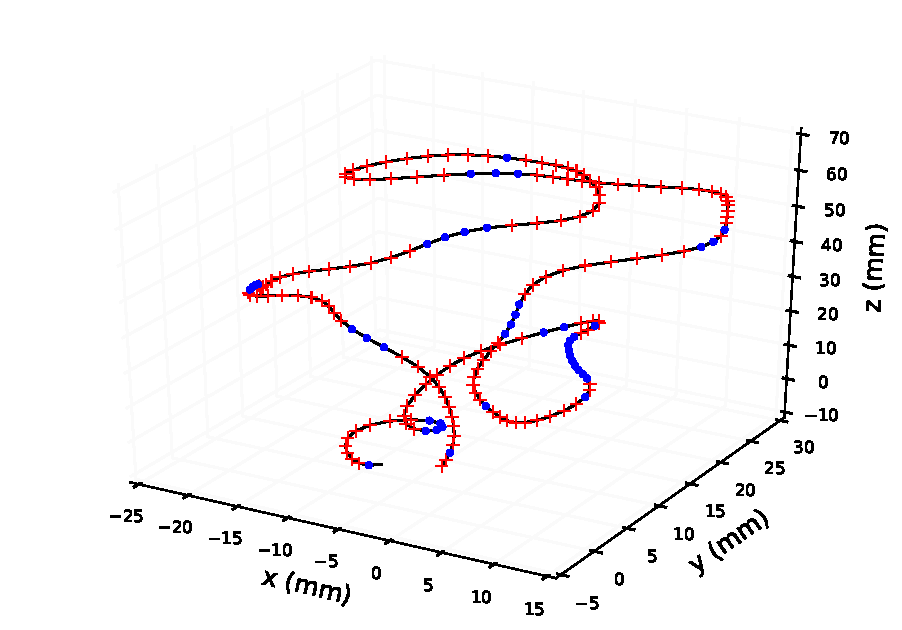
\includegraphics[scale=0.48]{fig/plt_trkcurv_nmagse2_6.pdf}
	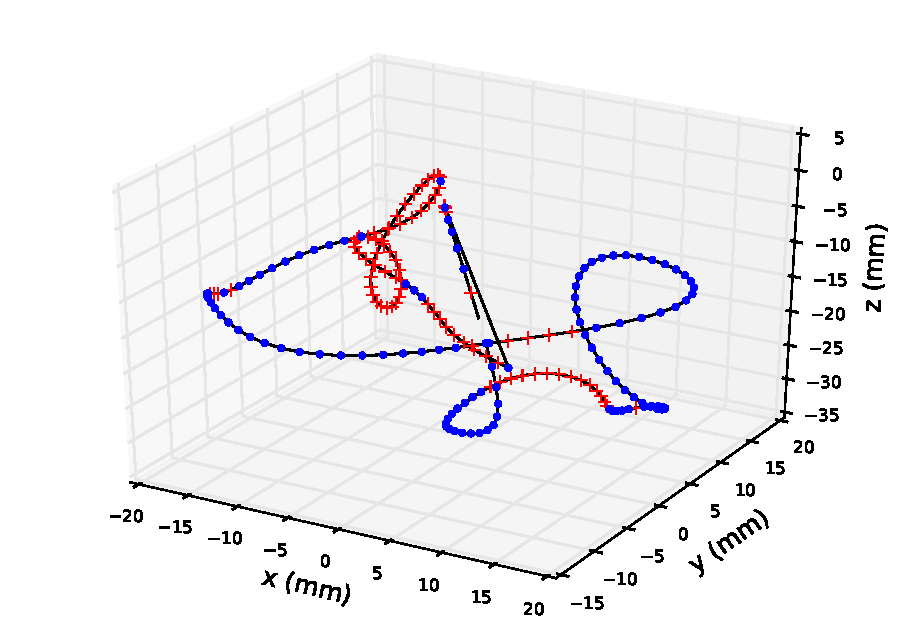
\includegraphics[scale=0.48]{fig/plt_trkcurv_nmagbb2_2.pdf}
	\caption{\label{fig_trkcurv}Calculated curvature sign at each point along the track for a single-electron event (left) and a double-beta event (right).  The red $+$ markers indicate positive curvature, while the blue dots indicate negative curvature.}
\end{figure}

A curvature sign array is created consisting of values of either $+1$ or $-1$ depending on the sign of each value in the calculated curvature array.  The curvature asymmetry factor is defined as the average of the curvature sign array using elements in the first half of the track minus the average of the curvature sign array using elements in the second half of the track.

\begin{equation}\label{eqn_assym}
\phi_{C} = \frac{1}{N/2}\Biggl(\sum_{i=0}^{N/2-1}\mathrm{sgn}(\kappa_{i}) - \sum_{i=N/2}^{N}\mathrm{sgn}(\kappa_{i})\Biggr).
\end{equation}

\noindent Note that if the number of hits in the track is odd, the first term includes the first $(N-1)/2$ hits and
the second term includes the remaining $(N-1)/2 + 1$ hits.

\section{Results: Additional Background Rejection}
The asymmetry factor shown in equation \ref{eqn_assym} was calculated for each of 10000 single-electron and 10000 $0\nu\beta\beta$ tracks per configuration for all combinations of $P =$ 5, 10, and 15 atm and $B =$ 0.1, 0.3, 0.5, 0.7, and 1.0 T.  In all of these configurations, the hits were smeared in $(x,y)$ with $\sigma_{s} = 2$ mm and sparsed with $N_{s} = 2$.  A cut on the calculated asymmetry factors defining what events were considered to be candidate $0\nu\beta\beta$ tracks was varied, and in each case the fraction of single-electron (background) events rejected by the cut was determined along with the fraction of $0\nu\beta\beta$ (signal) events accepted.  An example of such an analysis is summarized in figure \ref{fig_svsbg}.

\begin{figure}[!htb]
	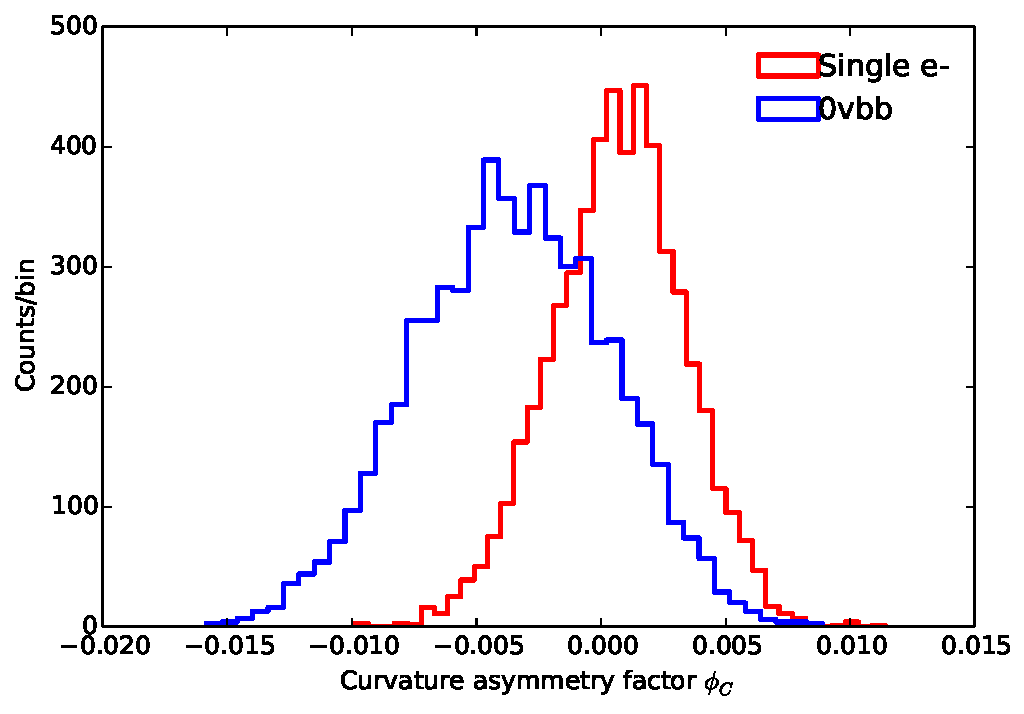
\includegraphics[scale=0.44]{fig/10atm_05T_scurv_diff_means.pdf}
	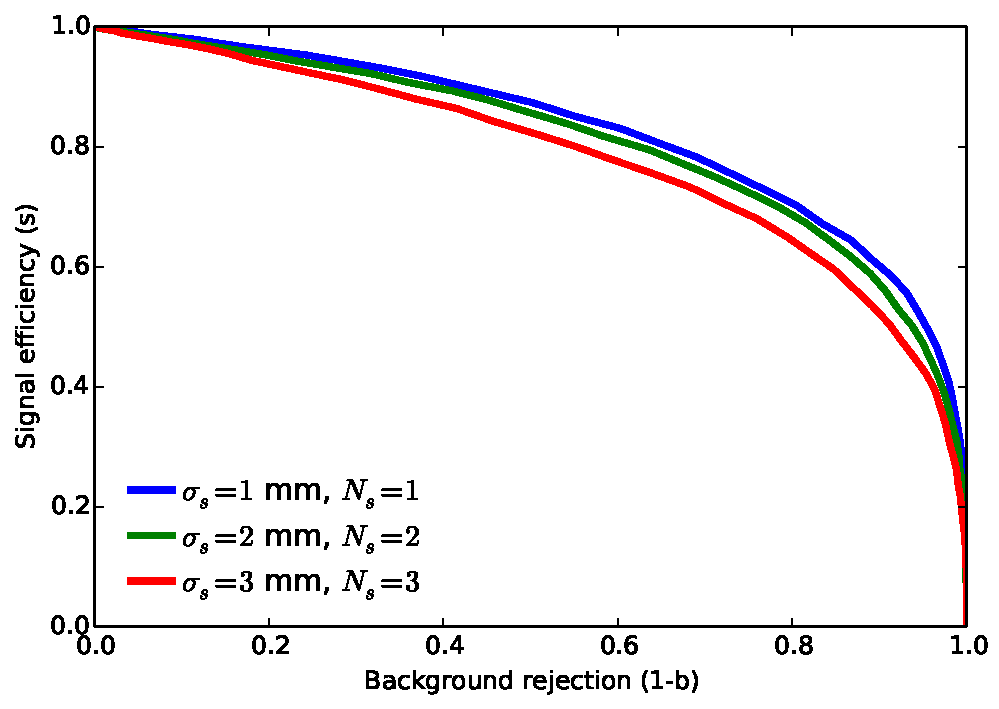
\includegraphics[scale=0.44]{fig/10atm_05T_sigvsb_all.pdf}
	\caption{\label{fig_svsbg}Curvature asymmetry factor for single-electron and $0\nu\beta\beta$ events (left) and resulting signal efficiency vs. background rejection curve produced by varying a cut on $\phi_{C}$ space (right).  These results were obtained for $P = 10$ atm and $B = 0.5$ T.}
\end{figure}

To demonstrate the performance of the method at the different configurations of gas pressure and magnetic field, we examine the signal efficiency obtained given 80\% background rejection.  The results are shown in figure \ref{fig_config}.

\begin{figure}[!htb]
	\centering
	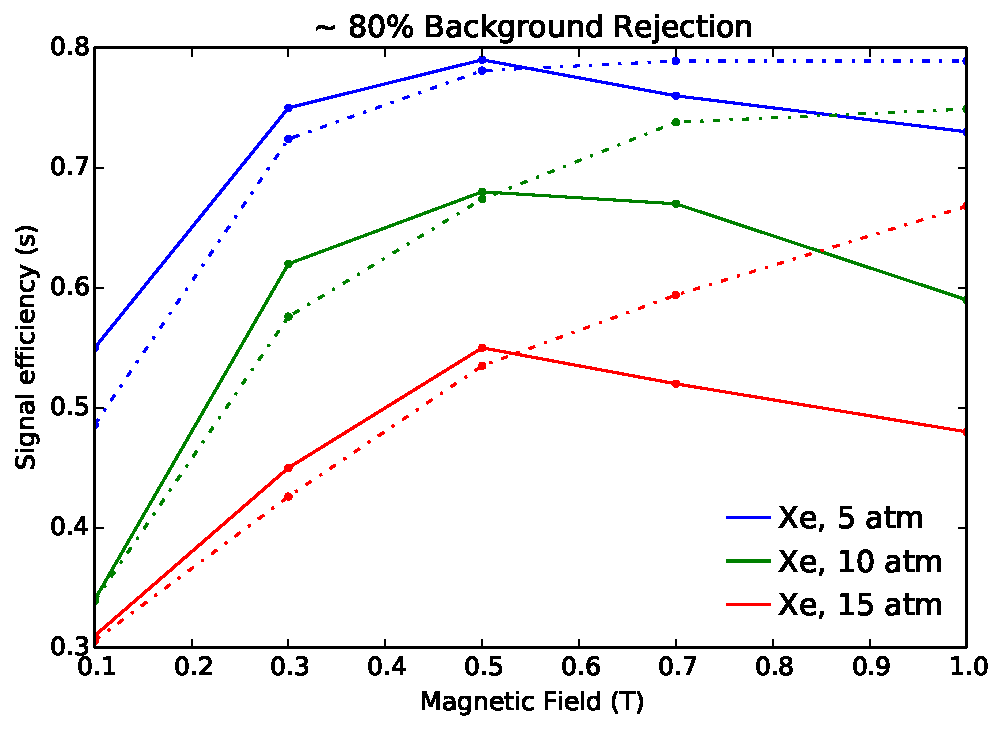
\includegraphics[scale=0.43]{fig/eff_vs_b_80.pdf}
	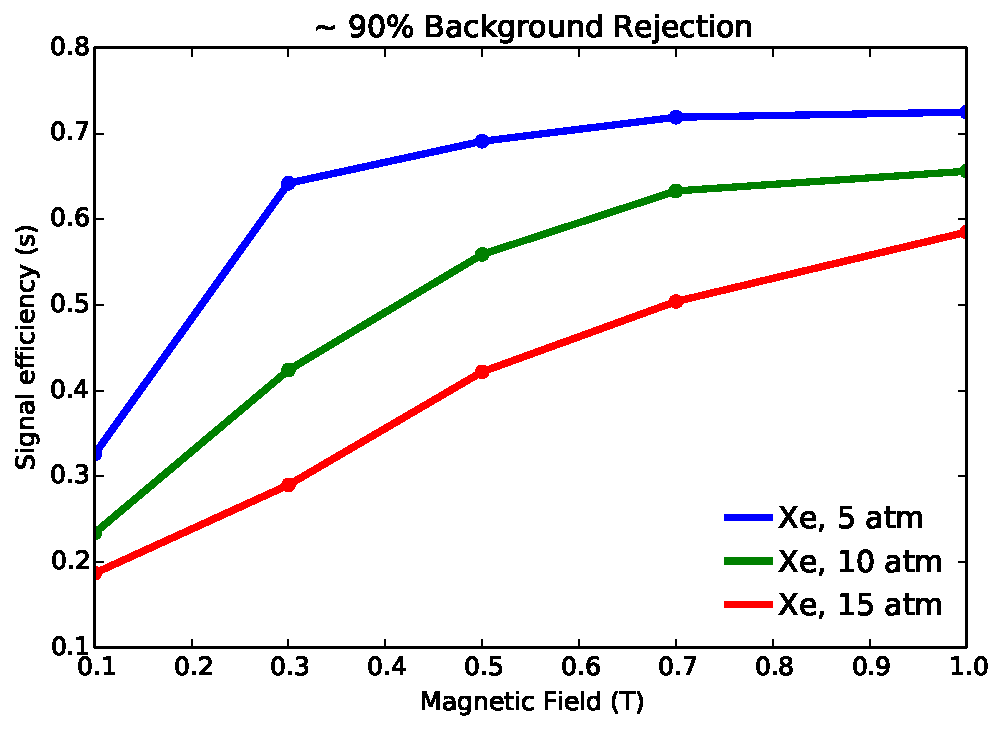
\includegraphics[scale=0.43]{fig/eff_vs_b_90.pdf}
	\caption{\label{fig_config}Signal efficiency corresponding to 80\% background rejection (left) and 90\% background rejection (right) vs. magnitude of applied external magnetic field for different pressures (NOTE: This needs to be updated to consider only the curvature method - it currently includes the KF analysis).}
\end{figure}

%Show signal vs. background separation (should we be using different training and run datasets?) for different configurations and related plots; 80 pct and 90 pct signal efficiency factors vs. B-field for different pressures; final conclusions and recommendations

\section{Conclusions}
The application of an external magnetic field in a high-pressure xenon detector capable of particle track reconstruction with resolution of approximately 2 mm in $(x,y,z)$ could present an additional background rejection factor of 80\% with an acceptable loss of signal efficiency at pressures less than about 10 atm.  The background rejection improves with decreasing pressure due to the more extended tracks produced at lower gas densities.  The use of this analysis at pressures above 10 atm does not seem practical due to the shortened tracks.  For a given pressure, there appears to be an optimal value of the magnetic field at which a maximum in signal efficiency is obtained for a given background rejection, and magnetic fields in the range of 0.4 - 0.8 T seem to give the best results.



(Additional comments on how this will apply to NEXT)

%\newpage % Please avoid layout-changing commands if not strictly necessary

%\begin{figure}[tbp] % figures (and tables) should go top or bottom of
%                    % the page where they are first cited or in
%                    % subsequent pages
%\centering
%\includegraphics[width=.4\textwidth]{fig.png}
%\caption{Caption.}
%\label{fig:xxx}
%\end{figure}

%\begin{table}[tbp]
%\caption{Caption.}
%\label{tab:xxx}
%\smallskip
%\centering
%\begin{tabular}{|lc|}
%\hline
%a&b\\
%c&d\\
%\hline
%\end{tabular}
%\end{table}


\acknowledgments

This work was supported by the European Research Council under the Advanced Grant 339787-NEXT and the Ministerio de Econom\'{i}a y Competitividad of Spain under Grants CONSOLIDER-Ingenio 2010 CSD2008-0037 (CUP), FPA2009-13697-C04-04, FPA2009-13697-C04-01, FIS2012-37947-C04-01, FIS2012-37947-C04-02, FIS2012-37947-C04-03, and FIS2012-37947-C04-04.

\bibliography{nextb}

\end{document}
